\section{Results of the Traditional Approach}
The proposed approach has been evaluated on two data sets. One is the AMI database \cite{AMI}, which consists of 175 ear images; and the other is the IIT Delhi database \cite{IIT}, which consists of 494 images of 125 distinct persons. The images were all converted to gray- scale images for ease of work. It has also been found out that contrast enhancement is an important factor for feature detection and matching, because it makes the feature detectors find better set of keypoints and increase the effectiveness of matching.
According to the experiments performed, it has been found that upper helix, antihe- lix, and tragus are the most important regions for feature selection compared to others. These regions contribute to about 64{\%} of the feature points.
Figure 7 shows some sample images from the two databases we used for our exper- iments. The graphs in Figure 8 indicates the average number of keypoints found and matched by SIFT and SURF detectors when the images are rotated from a range of 0 to 180 degrees. The results suggest that the SIFT detector is fairly stable over a variation of angles from 20 to 160 degrees, whereas the SURF detector, though faster and rotation invariant, is not very stable.
Table 1 shows the keypoints detected and matched by the SIFT and SURF detectors, where the performance ratio is the ratio of the number of matched points to that of detected features. It is obvious that the SIFT algorithm performs better when the sizes of images are decreased, while the SURF algorithm performs better when the image sizes are increased. However, the amount of detected keypoints by the SIFT detector is always higher than that by the SURF detector.

\begin{table}[]
\centering
\caption{SIFT and SURF detection and matching results at different scales}
\label{table1}
\begin{tabular}{lllllllllll}
\hline
\multicolumn{1}{c}{Scaling} &           
\multicolumn{1}{c}{Methods} &          
\multicolumn{1}{c}{0.25} &     
\multicolumn{1}{c}{0.5} &     
\multicolumn{1}{c}{0.75} &     
\multicolumn{1}{c}{1.0} &     
\multicolumn{1}{c}{2.0} &     
\multicolumn{1}{c}{3.0} &     
\multicolumn{1}{c}{4.0} &       \\ \cline{1-2}
\hline
 Number of Features & SIFT  & 28  & 53  & 58 & 64 & 170  & 247  & 233   \\
 & SURF & 3  & 12  & 30 & 41 & 39 & 41 & 44   \\
 \hline
  Number of Matches & SIFT  & 24  & 45  & 54 & 64 & 53  & 47  & 51   \\
 & SURF & 2  & 9  & 23 & 41 & 20 & 21 & 16   \\
 \hline
 Performance Ratio & SIFT  & 0.85  & .85  & 0.89 & 1.0 & 0.32 & .20 & 0.22  \\
 & SURF & 0.67 & 0.75  & 0.75 & 1.0  &  0.51 & 0.51 & .30  \\
 \hline
\end{tabular}
\end{table}

\begin{table}[]
\centering
\caption{Experimental results on the IIT Delhi database}
\label{table2}
\begin{tabular}{lllllll}
\hline
\multicolumn{1}{c}{Method} &           
\multicolumn{1}{c}{Number of Images} &          
\multicolumn{1}{c}{Matched } &     
\multicolumn{1}{c}{Unmatched } &     
\multicolumn{1}{c}{Time} &     
\multicolumn{1}{c}{Recognition Rate} &     \\ \cline{1-2}
\hline
SIFT  & 125  & 121  & 4 & 0.21 & 96.8 {\%}  \\
\hline
SURF & 125  & 118  & 7 & 0.183 & 94.4 {\%}    \\
 \hline

\end{tabular}
\end{table}

Table 2 shows an overview of how the two detectors work in real-life conditions where some images are not matched due to illumination changes as those images were mostly taken at night and at different angles. Thus, the descriptors fail to find enough feature keypoints for matching. The overall recognition rates of the SIFT and SURF algorithms on the IIT Delhi database are 96.8{\%}and 94.4{\%}, respectively. As a comparison, we also implemented other methods for ear recognition. The template matching technique yields a recognition rate of 93 {\%} for \cite{ansari}, and 92.6 {\%} for \cite{birbhanu}, whereas the recognition rate by the contour extraction technique \cite{bowyer} is 85 {\%} It is evident that the proposed technique yields a higher recognition rate.

\begin{table}[]
\centering
\caption{Einal Results after the outlier detection}
\label{table3}
\begin{tabular}{llllll}
\hline
\multicolumn{1}{c}{Method} &           
\multicolumn{1}{c}{Number of Images} &          
\multicolumn{1}{c}{Matched } &     
\multicolumn{1}{c}{Unmatched } &        
\multicolumn{1}{c}{Recognition Rate} &     \\ \cline{1-2}
\hline
SIFT  & 125  & 119  & 6  & 95.2 {\%}  \\
\hline
SURF & 125  & 114  & 11  & 91.2 {\%}    \\
 \hline

\end{tabular}
\end{table}

From the above table \ref{table3}, it can be seen that due the removal of outliers - the number of false matches have decreased to a certain extent. Thus, the false matches have been successfully removed keeping in mind that the noise in the image is gaussian, the performance of the algorithm decreases but the algorithm is robust and thus is more favourable than the previous approach.

\begin{figure}
	\DeclareGraphicsExtensions{.pdf,.png,.jpg}
		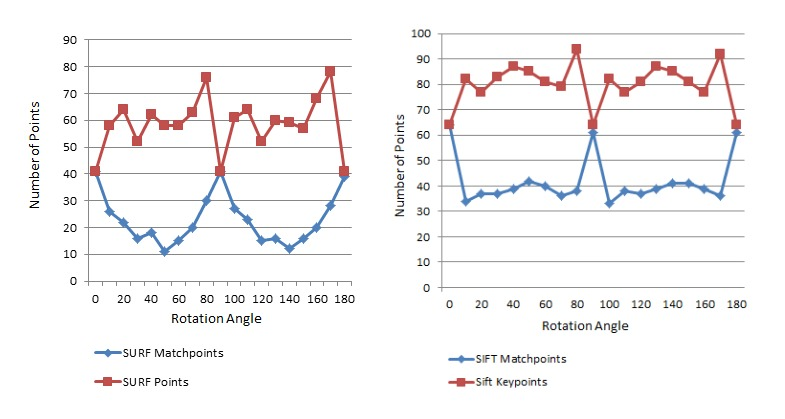
\includegraphics[width=\textwidth]{Figures/Figure17}
	\caption{A comparison result of the detected and matched keypoints by SURF and SIFT}
	\label{fig:Figure13}
\end{figure}

\begin{figure}
	\DeclareGraphicsExtensions{.pdf,.png,.jpg}
	\begin{center}
		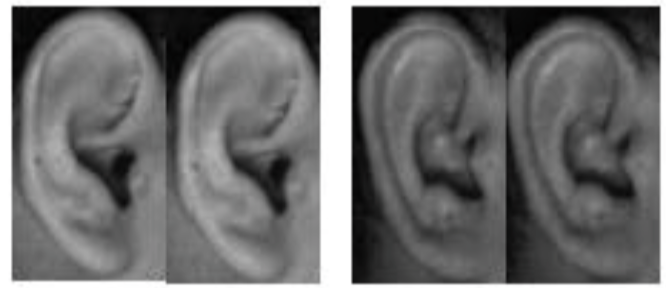
\includegraphics[width=0.5\textwidth]{Figures/Figure13}
	\end{center}
	\caption{Sample Images from IIT Delhi Ear Dataset}
	\label{fig:Figure13}
\end{figure}

\begin{figure}
	\DeclareGraphicsExtensions{.pdf,.png,.jpg}
	\begin{center}
		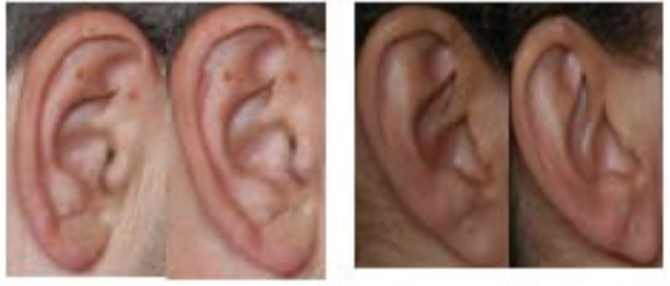
\includegraphics[width=0.5\textwidth]{Figures/Figure14}
	\end{center}
	\caption{Sample Images from AMI Ear Dataset}
	\label{fig:Figure14}
\end{figure}